\documentclass{scrartcl}

%Configuración de página

\KOMAoptions{fontsize=12pt,
	parskip=true,
	paper=letter
}



%Margenes 
\usepackage[left=2.54cm,
right=2.54cm,
top=2.54cm,
bottom=2.54cm,
footskip=1cm,
headsep=1cm]{geometry}

%Paquetes cargados
\usepackage[spanish]{babel}
\usepackage{amsmath,amssymb}
\usepackage{array}
\usepackage{xcolor}
\usepackage{tabularray}
\usepackage{graphicx}
\usepackage{rotating}
\usepackage[headsepline=true,footsepline=true]{scrlayer-scrpage}

%Uso de tikz

\renewcommand{\sectionmark}[1]{\markright{\thesection\ #1}}

\lohead{\rightmark}
\cohead{}
\rohead{\pagemark}

\lofoot{}
\cofoot{}
\rofoot{Ing. Ervin Adrian Duran Aguilar}


\title{Cuadernillo de Ejercicios}
\author{Ing. Ervin Adrian Duran Aguilar}
\date{}

\begin{document}
	\maketitle
	\section{Secuenciales}
	
	\begin{enumerate}
		
		\item Pedir 2 números al usuario y sumarlos, restarlos, multiplicarlos y dividirlos.
		
		\item Convertir Grados Celsius a Grados Fahrenheit.
		
		\item Sacar la hipotenusa de un triángulo rectángulo, pidiendo al usuario el valor de los 2 catetos.
		
		\item Hacer un Programa que calcule longitudes de Circunferencia.

		\item Hacer un Programa que calcule áreas de trapecios.
		
		\item Calcule la media aritmética de 3 números cualesquiera.
		
		\item Una tienda ofrece un descuento del 15\% sobre el total de la compra y un cliente desea saber cuánto deberá pagar finalmente por su compra.
		
		\item Dadas las horas trabajadas de una persona y el valor por hora. Calcular su
		salario e imprimirlo.
		
		\item Calcular el nuevo salario de un obrero si obtuvo un incremento del 25% sobre
		su salario anterior.
		
		\item Un alumno desea saber cuál será su calificación final en la materia de	Algoritmos. Dicha calificación se compone de los siguientes porcentajes:
		
			\begin{itemize}
					\item 55\% del promedio de sus tres calificaciones parciales.
					\item 30\% de la calificación del examen final.
					\item 15\% de la calificación de un trabajo final. (Propuesto)				
			\end{itemize}

		\item Calcular la cantidad de segundos que están incluidos en el número de horas,
		minutos y segundos ingresados por el usuario.
		
		\item Hacer un Programa que obtenga la media geométrica de tres numeros.
		
		\item Un maestro desea saber que porcentaje de hombres y que porcentaje de		mujeres hay en un grupo de estudiantes.
		
		\item Volumen y Área de un Cubo.
		
		\item Tres personas deciden invertir su dinero para fundar un empresa. Cada una de ellas invierte una cantidad distinta. Obtener el porcentaje que cada quien invierte con respecto a la cantidad total invertida.
		
		\item Volumen y Área de una Esfera.	
		
		\item Dado un numero de 4 dígitos halle la suma de dígitos en la posición par y el producto de los dígitos en la posición impar. Par ello realice el conteo de izquierda a derecha de los dígitos.
		
		\begin{table}[ht]
			\centering
			\begin{tblr}{
				hlines,vlines
			}
				$1^{\circ} $& $2^{\circ}$  & $3^{\circ}$  & $4^{\circ}$  \\
				8 & 4 & 7 & 5 \\
			\end{tblr}
		\end{table}
	
		Suma = 17
		Producto = 20
		
		\item Realizar el análisis, diagrama de flujo y prueba de escritorio, para calcular y visualizar el área y el volumen de la siguiente figura:
		
			\begin{minipage}{0.4\textwidth}
				%\begin{figure}[ht]
					\centering
					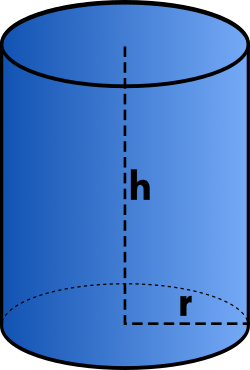
\includegraphics[scale=0.3]{img/cilindro.png}
				%\end{figure}
			\end{minipage}
			\begin{minipage}{0.5\textwidth}
				\centering
				$A=2 \pi r(h+r)$
				$$V=\pi r^{2} h$$
			\end{minipage}
		
		\item Diseñar un programa para calcular el volumen de la siguiente figura y visualizar el resultado. Formulas generales:
		
			\begin{minipage}{0.4\textwidth}
				%\begin{figure}[ht]
				\centering
				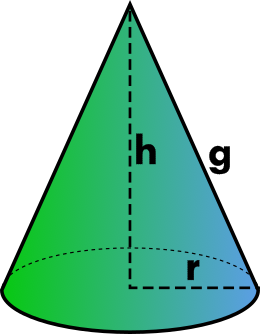
\includegraphics[scale=0.3]{img/cono.png}
				%\end{figure}
			\end{minipage}
			\begin{minipage}{0.5\textwidth}
				\centering
				$A_{total}= \pi r^{2} + \pi r g$
				$$V=\frac{\pi r^{2} h}{3}$$
			\end{minipage}
		
		\item Realizar un programa para introducir un número entero de 5 dígitos por teclado, realizar el proceso para invertirlo.
		
		Ejemplo: 64532 →23546
		
		\item Hacer leer un numero A, evaluar sucesivamente las expresiones siguientes y desplegar los resultados obtenidos:
		
		\begin{itemize}
			\item [a)] $B=A-200$
			\item [b)] $C=4\cdot B+B-A$
			\item [c)] $D=A-B+C/4$
		\end{itemize}
		

		
		
		\item Hacer leer S en segundos, convertir a minutos y horas. Desplegar los resultados.
		
		\item Determinar la hipotenusa de un triángulo rectángulo conocidas las longitudes de sus dos catetos.
		
		\item Se introduce a través del teclado 3 valores enteros en las variables A, B, C. Diseñar el algoritmo para calcular la suma, el producto y la media de los tres números y visualizar los resultados.
		
		\item Hacer un programa en el que ingresados dos números por la pantalla se debe calcular la suma, diferencia, producto y división de los mismos.
		
		\item Calcule el total de una factura de servicio telefónico, de acuerdo a la cantidad de minutos consumidos de llamadas a teléfono fijo(0.20 Bs. el minuto) y minutos consumidos de llamadas a teléfono móvil (0.80 Bs. el minuto), y un descuento del 5\% para las llamadas a teléfono móvil.
		
		\item Todos los lunes, miércoles y viernes, una persona corre la misma ruta y cronometra los tiempos obtenidos. Determinar el tiempo promedio que la persona tarda en recorrer la ruta en una semana cualquiera.
		
		\item Un maestro desea saber qué porcentaje de hombres y que porcentaje de mujeres hay en un grupo de estudiantes.
		
		\item Suponga que un individuo desea invertir su capital en un banco y desea saber cuánto dinero ganara después de un mes si el banco paga a razón de 2\% mensual.
		
		\item Escribir un programa para convertir una medida dada en pies a sus equivalentes en:
		
			\begin{enumerate}
				\item Yardas
				\item Pulgadas
				\item Centímetros
				\item Metros
			\end{enumerate}

		\item Tres personas deciden invertir su dinero para fundar una empresa. Cada una de ellas invierte una cantidad distinta. Obtener el porcentaje que cada quien invierte con respecto a la cantidad total invertida.
		
		\item Escribir un programa para calcular y visualizar el área de la siguiente figura, considerar que el circulo que se encuentra en medio es un hueco en medio del triángulo que es de tipo rectángulo.
		
		\begin{figure}[ht]
			\centering
			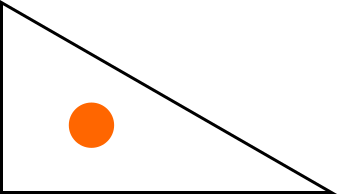
\includegraphics[scale=0.5,angle=-45]{img/triangulo.png}
		\end{figure}
		
		\item Escribir un programa que permita calcular el precio de venta de un producto considerando que debe incrementar el 20\% del costo de proveedor y 5 porciento por costos de distribución. 
		
		Por ejemplo:\\
		Costo de proveedor = 50\\
		Precio de venta es = 50 + 10+ 2,5 = 62,5
		
		\item Una empresa constructora vende terrenos con la forma de la figura. Obtener el área
		respectiva de un terreno de medidas de cualquier valor.
		
		\begin{figure}[ht]
			\centering
			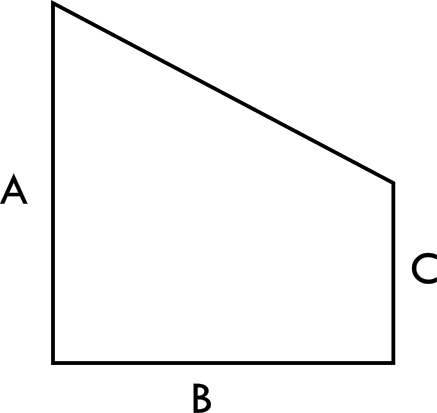
\includegraphics[scale=0.4]{img/1.png}
		\end{figure}
		
		\item Se requiere obtener la distancia entre dos puntos en el plano cartesiano, tal y como se muestra en la figura. Obtener la distancia entre esos puntos.
		
		\begin{figure}[ht]
			\centering
			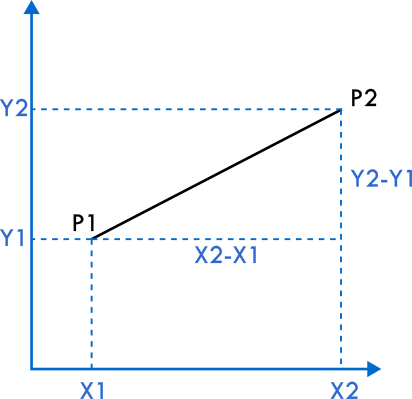
\includegraphics[scale=0.4]{img/2.png}
		\end{figure}
		
		\item Epsas requiere determinar el pago que debe realizar una persona por el total de metros cúbicos que consume de agua al llenar una alberca (ver figura). Determinar ese pago.
	
		\item Un comerciante desea saber cual es el precio al que debe que debe promocionar sus productos los cuales venderá con factura. Para ello tiene el precio al que adquiere cada producto y al que debe adicionar el 16\% para hallar el precio de venta.
		
		\item Las poblaciones tienden a expandirse exponencialmente. Esto es 
		\begin{equation*}
			P = P_{0}e^{rt}
		\end{equation*}
		
		donde:
		\begin{eqnarray*}
			P		   &=&	\mbox{población actual} \\
			P_{o}  &=& \mbox{Población original} \\
			r 			& = & \mbox{Tarifa de crecimiento continua, expresado como fracción}\\
			t 			& = & \mbox{tiempo}
		\end{eqnarray*}
		
		Si originalmente se tienen 100 conejos que se reproducen a una tasa de crecimiento constante de 90\% (r = 0.9) por año, encuentre cuántos conejos tendrá al final de 10 años.
		
		\item Las tasas de reacción química son proporcionales a una constante de tasa $k$ que cambia con la temperatura de acuerdo con la ecuación Arrhenius
		
		\begin{equation*}
			k = k_{0} e^{-\frac{Q}{RT}}
		\end{equation*}
		
		Para cierta reacción
		
		\begin{eqnarray*}
			Q  &=&	800\;cal/mol \\
			R  &=&  1.987\;cal/mol\;K \\
			k_{0} &=& 1200\;min^{-1} \\
		\end{eqnarray*}
		
		Encuentre los valores de $k$ para temperaturas desde $100\;K$ hasta $500\;K$, en incrementos de $50\;grados$. Cree una tabla con sus resultados.
	\end{enumerate}

	\section{Estructuras Condicionales}
		
	\begin{enumerate}
		
		\item Determinar si un alumno aprueba o reprueba un curso, sabiendo que aprobara si su promedio de tres calificaciones es mayor o igual a 10.5; reprueba en caso contrario.
		
		\item Mostrar el resultado de la suma de 2 números enteros, si esta supera a 10.
		
		\item Determinar si un número es par, impar o cero.
		
		\item Dado 3 números Calcular el Mayor.
		
		\item Ingrese 2 números desde el teclado e imprima solo los positivos.
		
		\item Un obrero necesita calcular su salario semanal, el cual se obtiene de la
		siguiente manera:
		
			\begin{itemize}
				\item Si trabaja 40 horas o menos se le paga \$16 por hora
				\item Si trabaja más de 40 horas se le paga \$16 por cada una de las primeras 40 horas
				y \$20 por cada hora extra.		
			\end{itemize}
		
		
		\item Ingresar por teclado el nombre y el signo de cualquier persona e imprima, el
		nombre solo si la persona es signo Aries.
		
		\item Ingresar por teclado el nombre, la edad y el sexo de cualquier persona e	imprima, solo si la persona es de sexo masculino y mayor de edad, el nombre de la persona.
		
		\item Hacer un algoritmo que calcule el total a pagar por la compra de camisas. Si se compran tres camisas o más se aplica un descuento del 20\% sobre el total de la compra y si son menos de tres camisas un descuento del 10\%
		
		\item En un supermercado se hace una promoción, mediante la cual el cliente		obtiene un descuento dependiendo de un número que se escoge al azar. Si el		numero escogido es menor que 74 el descuento es del 15\% sobre el total de la compra, si es mayor o igual a 74 el descuento es del 20\%. Obtener cuanto		dinero se le descuenta.
		
		\item Calcular el total que una persona debe pagar en una llantera, si el precio de cada llanta es de \$800 si se compran menos de 5 llantas y de \$700 si se compran	5 o más.
		
		\item En un almacén se hace un 20\% de descuento a los clientes cuya compra
		supere los S/. 1000 ¿Cuál será la cantidad que pagara una persona por su
		compra?
		
		\item Ecuaciones de Segundo Grado: $Ax^2 + Bx + C$.
		
		\item Hacer un programa que lea 2 números, y los imprima en forma ascendente.
		
		\item Hacer un programa que simule el lanzamiento de una moneda.
		
		\item Una distribuidora de motocicletas tiene una promoción de fin de año que consiste en lo siguiente. Las motos marca Honda tienen un descuento del 5\%, las	marcas Yamaha del 8\% y las Suzuki del 10\%, las otras marcas 2\%.
		
		\item En una tienda de descuento se efectúa una promoción en la cual se hace un descuento sobre el valor de la compra total según el color de la bolita que el 	cliente saque al pagar en caja. Si la bolita es de color blanco no se le hará 	descuento alguno, si es verde se le hará un 10\% de descuento, si es amarilla un 25\%, si es azul un 50\% y si es roja un 100\%. Se sabe que solo hay bolitas de los colores mencionados.
		
		\item Hacer un programa que pida tres números y detecte si se han introducido en
		orden creciente.
		
		\item Hacer un programa que pida tres números e indicar si el tercero es igual a la suma del primero y el segundo.
		
		\item Hacer un programa Que tome tres números y diga si la multiplicación de los
		dos primeros es igual al tercero.
		
		\item Que lea una hora en hora:minutos:segundos y diga la hora que es un segundo
		después.
		
		\item Hacer un programa que tome dos números y diga si ambos son pares o
		impares.
				
		\item Se requiere realizar un programa que determine si un estudiante es apto o no. Un estudiante es apto si su nota finar es mayor a 5,1 y no apto caso contrario. La nota finalse calcula a partir de la nota de Trabajos, Test y examen con la siguiente ponderación:
		
		Nota Final = 0.3* Trabajos + 0,5 * Test + 0,3 *Examen.
		
		\item Una empresa Telefónica desea implementar un algoritmo que calcule el costo de las llamadas de sus usuarios para ello el dato que se tiene es el tiempo total de una llamada en segundos, para ello el algoritmo debe realizar lo siguiente:
		
		a) Convertir los segundos a minutos.
		b) Si la llamada tuvo más de un minuto se cobrará 2 Bs el primer minuto y los
		siguientes minutos cada una a 0, 50 ctv. Ojo si hay segundos extras se los
		minutos se los debe considerar como “ La Yapa”
		c) El algoritmo debe mostrar como resultado el costo total de la llamada.
		
		\item Escribir un programa para calcular y visualizar el área de la siguiente figura, considerar que el circulo que se encuentra en medio es un hueco en medio del triángulo que es de tipo rectángulo. Si el diámetro del hueco es mayor que alguno de los lados entonces enviar un mensaje que indique que no se puede calcular el área.
		
		\item Escribir un programa que permita diagnosticar los resultados de una prueba de COVID. Los resultados obtenidos son valores numéricos para los anticuerpos IgM e IgG que, según los rangos de referencia se interpretan cómo positivos o negativos para cada uno de los dos anticuerpos. Para el programa considere la siguiente tabla:
		
		\begin{table}[ht]
			\centering
			\begin{tblr}{X[2,c]X[4,l]}
					\hline
					Valor de IgM y IgC & Resultado del programa \\
					Resultado > 1.1  &  
					\hline
					Este es un resultado positivo. Cualquier valor por encima de este número debe interpretarse como positivo. Tenga en cuenta que valores mayores no significan mayor inmunidad ni mayor o menor tiempo de infección. Los resultados deben ser interpretados en conjunto con su médico. \\
					\hline
					Resultado < 0.9:  &
				
					Este es un resultado negativo. Cualquier valor
					por debajo de este número debe interpretarse
					como negativo. \\
					\hline
					Resultado entre 0.9 y 1.1 &
					Es indeterminado. El resultado no es claro. Le
					recomendamos repetir el examen en 5 o 7 días. \\
					\hline
			\end{tblr}
		\end{table}
	
		\item Escribir un programa que permita diagnosticar a un paciente que evalué su presión arterial según la siguiente tabla, considere que debe ingresar la medición sistólica y diastólica.
		
			\begin{table}[ht]
			\centering
			\begin{tblr}{hlines,vlines}
					Diagnóstico & Sistólica & Diastólica \\
					Óptima & <120 & <80 \\
					Normal & 120-129 & 80-84\\
					Normal-Alta & 130-139 & 85-89\\
					Hipertensión  leve 1 & 140-159 & 90-99 \\
					Hipertensión Moderada & 160-179 & 100-109 \\
					Hipertención severa & $\ge$ 180& $\ge$ 110 \\
			\end{tblr}
		\end{table}
		
		\item Realice un algoritmo para determinar el sueldo semanal de un trabajador con base en las horas trabajadas y el pago por hora, considerando que después de las 40 horas cada hora se considera como excedente y se paga el doble.
		
		\item El director de una escuela está organizando un viaje de estudios, y requiere determinar cuánto debe cobrar a cada alumno y cuánto debe pagar a la compañía de viajes por el servicio. La forma de cobrar es la siguiente: si son 100 alumnos o más, el costo por cada alumno es de \$65.00; de 50 a 99 alumnos, el costo es de \$70.00, de 30 a 49, de \$95.00,y si son menos de 30, el costo de la renta del autobús es de \$4000.00, sin importar el número de alumnos. Determinar el pago a la compañía de autobuses y lo que debe pagar cada alumno por el viaje.
				
		\item Fábricas “El cometa” produce artículos con claves (1, 2, 3, 4, 5 y 6). Se requiere un algoritmo para calcular los precios de venta, para esto hay que considerar lo siguiente:
		
			\begin{itemize}
				\item Costo de producción = materia prima + mano de obra + gastos de fabricación.
				\item Precio de venta = costo de producción + 45\% de costo de producción.
			\end{itemize}
		
		El costo de la mano de obra se obtiene de la siguiente forma: para los productos con clave 3 o 4 se carga 75\% del costo de la materia prima; para los que tienen clave 1 y 5 se carga 80\%, y para los que tienen clave 2 o 6, 85\%.
		
		Para calcular el gasto de fabricación se considera que, si el artículo que se va a producir tiene claves 2 o 5, este gasto representa 30\% sobre el costo de la materia prima; si las claves son 3 o 6, representa 35\%; si las claves son 1 o 4, representa 28\%. La materia prima tiene el mismo costo para cualquier clave.
		
		\item Desarrollar un algoritmo que permita leer tres números A, B y C y se desea calcular el valor de una variable D considerando lo siguiente:
		
		Si A=B, entonces evaluar si A>C y si cumple esta condición hallar D=A 2, sino D=C2. Si A es diferente de B entonces evaluar si A>B y si cumple esta condición hallar D=A-10, sino D=B+10. Finalmente imprimir el valor de D.
		
		\item Desarrollar un algoritmo que permita leer el código de la fruta e imprimir la sub-categoría y nombre de la fruta de acuerdo a la siguiente tabla (en la tabla no figuran todas las frutas):
		
		Por ejemplo, si el código de fruta ingresado es 230 entonces se debe imprimir como
		resultado “Semiácida” y “mandarina”, esto porque:
		230
		Nota. El ejercicio debe ser resuelto haciendo uso del manejo de dígitos.
		
		\item Diseñar un programa para hallar el mayor de 2 números.

		\item Diseñar un programa para el ingreso a una discoteca el cual verifique la edad y envié un mensaje (“BIENVENIDO”) caso contrario (“ACCESO DENEGADO”).
		
		\item Diseñar un programa que determine si un número es múltiplo de 3 y de 5. Por ejemplo, si el número introducido es 9, se deberá mostrar un mensaje que indique “No es múltiplo	de 3 y de 5”; si se introduce el número 30 se mostrará un mensaje que indique “Si es múltiplo de 3 y 5”.
		
		\item Leer tres calificaciones de un postulante a la carrera de INGENEIRIA DE SISTEMAS en	la materia Introducción a la Informática. Diseñar un algoritmo para averiguar si el alumno aprueba o reprueba la materia. Considerar que para aprobar la nota promedio debe ser mayor o igual a 51.
		
		\item Dado 3 números mostrarlos de forma ordenada descendente. Por ejemplo, si se
		introduce los números 5, 2, 13; se mostrará 13, 5, 2.
		
		\item Diseñar un programa que permita determinar si un número es positivo, negativo o neutro.
		
		\item Dados tres números determinar si la suma de una pareja de ellos es igual al tercer número, si se cumple la condición presentar mensaje “iguales” caso contrario “distintos” y finalizar.
		
		\item Hacer leer dos números A y B, del mayor restarle el menor. Desplegar el resultado.
		
		\item Dado un número entero P, si P es mayor 999 adicionarle la mitad de su valor, mostrar el nuevo número. Si P es mayor 99 y menor que 999 verificar si el número P es múltiplo de 6, si P es negativo convertirlo a positivo y dividir entre 10 dicho número, caso contrario mostrar el mensaje "no hago nada".
		
		\item Resuelva el siguiente problema: Leer dos números del teclado y multiplicarlos si son iguales, restarlos si el primero es mayor que el segundo o sumarlos si el primero es menor que el segundo.
	\end{enumerate}

\section{Estructura Repetitivas FOR-WHILE}
	
	\begin{enumerate}
		\item Suma de los n primeros números.
		\item Digite un número, si el numero supera a 10, multiplique los 10 primeros números, sino, súmelos.
		\item Múltiplos de 3 desde 1 hasta n.
		\item Múltiplos de 5 desde 1 hasta n.
		\item Sumar 1-2+3-4...
		\item Sumar pares desde n hasta m.
		\item Numero Primo
		\item Factorial de un número
		\item Suma de Factoriales.
		\item Serie Fibonacci
		\item Hacer un programa que imprima la suma de todos los números pares que hay	desde 1 hasta n, y diga cuantos números hay.
		\item Hacer un programa que imprima la suma de todos los números impares que	hay desde n hasta m, y diga cuantos números hay.
		\item Hacer un programa que pida dos números y muestre todos los números que	van desde el primero al segundo. Se debe controlar que los valores son correctos.
		\item Hacer un programa que pida dos números y sume todos los números que van	desde el primero al segundo. Se debe controlar que los valores son correctos.
		\item Hacer un programa que haga un menú del tipo “desea salir (S/N)” y el		programa no termine hasta que el usuario teclee “S”.
		\item Hacer un programa que calcule la suma de los cuadrados de los 100 primeros números.
		\item Hacer un programa que calcule la media de números.
		\item Hacer un programa que calcule la media de X números, se dejarán de solicitar números hasta que se introduzca el cero.
		
		\item Escribir un programa que imprima todos los números pares entre dos números que		se le pidan al usuario.
		
		\item Realizar un algoritmo que muestre la tabla de multiplicar hasta el 10, de un número		introducido por teclado.
		
		\item Leer un número y verificar si es un número perfecto.
		
		\item Una empresa les paga a sus empleados con base en las horas trabajadas en la semana. Realice un algoritmo para determinar el sueldo semanal de N trabajadores y, además, calcule cuánto pagó la empresa por los N empleados.
		
		\item Escribe un programa que, dados dos números, uno real (base) y un entero positivo (exponente), saque por pantalla el resultado de la potencia. No se puede utilizar el operador de potencia.
		
		\item Escribe un programa que diga si un número introducido por teclado es o no primo. Un número primo es aquel que sólo es divisible entre él mismo y la unidad.
		
		Nota: Es suficiente probar hasta la raíz cuadrada del número para ver si es	divisible por algún otro número.
		
		\item La compañía de luz DELAPAZ requiere determinar el pago que deben realizar los	N consumidores por el uso de energía eléctrica, la cual se mide en kilowatts por hora (KWH) y el costo por el consumo de KWH es de Bs. 0.73. Además, se debe considerar el pago por el alumbrado público y por el aseo urbano los cuales son Bs. 8.22 y 8.80, respectivamente. Imprimir el total que debe pagar cada consumidor y el monto total de las N transacciones.
		
		\item La ecuación canónica de una circunferencia centrada en el punto $(h, k)$ de coordenadas tiene la forma: $(x-h)^2 + (y-k)^2 = r^2$ donde r es el radio de dicha circunferencia. Crear un programa para leer N puntos y verificar cuantos de estos	puntos leídos se encuentran dentro de la circunferencia. Imprimir la cantidad y	cuáles son los puntos que se encuentran dentro de la circunferencia.
		
		\item Una fábrica produce mensualmente 5000 zapatos, se ha determino que vende en promedio 4730 zapatos. Actualmente tiene un depósito con una capacidad de 30000 de la cual ya esta ocupada un 20\%. En cuantos meses se llenará el depósito. Resolver utilizando la estructura repetitiva while (mientras)
		
		\item En una empresa se tiene un almacén de material de escritorio en el cual se han comprado 370 paquetes de hojas carta, los empleados de la empresa, solicitan de manera mensual las siguientes cantidades. RRHH: 3 paquetes, Sistemas: 4 paquetes, Financiera:7 paquetes, Administrativa: 12 paquetes, Gerencias: 3	paquetes. Determinar cuándo se tiene que renovar el inventario de papel carta si	no se debe tener menos de 30 paquetes almacenados.
		
		\item El gobierno ha establecido que el incremento del sueldo mínimo nacional deberá ser de 10\%cada año. Realizar un algoritmo que muestre el sueldo mínimo por los siguientes “N” años. El sueldo mínimo actual y N son variables de entrada.	Por ejemplo, si el sueldo mínimo actual es 1000, al terminar el primer año el sueldo será 1100, al terminar el segundo año será de 1210, etc.
		
		\item Realice un diagrama de flujo que permita calcular la nota más alta y la mínima un grupo de N estudiantes.
		
		\item Realice un diagrama de flujo que pida 7 números y calcula y muestra la suma de todos los primos.
		
		Por ejemplo. 1, 3, 4, 6, 11, 100, 9
		Suma = 1 + 3 + 11 = 15
		
		\item Construya un diagrama de flujo que pida N números naturales y mayores a 10 y menores a 100, y calcula y muestra la suma de todos pares.
		
		Por ejemplo. N=5 90 20 31 45 11
		Suma=90+20 = 110
		
		\item Lea un lote de números hasta que se introduzca un número negativo o el cero, y muestre la cantidad y suma de números primos y no primos que contenga.
		
		\item Lea un lote de números hasta que se introduzca un el cero, y de cada 3 números leídos halle y muestre su promedio.
		
		\item Dado un numero K entero mayor a 1000 rotar sus dígitos a la derecha X veces. Mostrar cada rotación
		
		Ejemplo: Si K = 3456 y X= 3:
		Las rotaciones son: 6345, 5634, 4563
		
		\item Escribe un programa que le pida al usuario un numero entre el 1 y el 9 - pediremos al usuario dicho número hasta que cumpla la condición- una vez introducido	correctamente el programa debe escribir la tabla de multiplicar de ese número usando un bucle for, después de escribir la tabla le preguntaremos ¿quieres introducir otro número? S/N si pulsa S, volveremos a pedirle otro número si pulsa N saldrá un mensaje dándole las gracias por usar nuestro programa y finalizara la ejecución, las tablas de los números que introduzca tendrán el siguiente formato de	salida: 7X1=7 7X2=14 ............. 7X9=63
		
		\item Escribe un programa que lea números enteros positivos hasta que se introduzca un 0. El programa deberá mostrar por pantalla la cantidad de números leídos, el mayor, el menor y la media de los números leídos.
		
		\item La conjetura de Ulam afirma que dado un entero y siguiendo los pasos siguientes siempre obtenemos un 1. • Si el número es par se divide por 2. • Si es impar se	multiplica por 3 y se suma 1. Escribe un programa que le pida al usuario un número	entero y que compruebe si la conjetura de Ulam es cierta, el programa deberá	escribir toda la secuencia hasta llegar al uno. Por ejemplo si el usuario introduce un	5 la secuencia sería: 5, 16, 8, 4, 2, 1.
		
		\item Dos números a y b se dice que son amigos si la suma de los divisores de a (salvo él mismo) coincide con b y viceversa. Diseña un programa que tenga como entrada dos números naturales y que indique mediante un mensaje si son amigos o no.
		
		\item Las empresas estatales han establecido que el incremento del sueldo mínimo nacional deberá ser de 12\% cada año. Realizar un algoritmo que muestre el sueldo mínimo por los siguientes “N” años. El sueldo mínimo actual y N son variables de entrada.	Por ejemplo, si el sueldo mínimo actual es 1000, al terminar el primer año el sueldo será 1120, al terminar el segundo año será de 1254.4, etc, mostrar para los N años.
		
		\item Dado un numero de mínimo 5 dígitos hallar la suma de sus dígitos pares y el
		producto de sus dígitos impares.
		Ejemplo: 86547
		Suma: 18
		Producto: 35
		\item Escribir un programa que visualice la siguiente salida:
		1
		1 2
		1 2 3
		1 2 3 4
		1 2 3
		1 2
		1
		
		\item Diseñar e implementar un programa que lea un total de R números y cuente el
		número de sus entradas que son positivos negativos y cero.
		
		\item Diseñar e implementar un programa que solicite a su usuario un valor no negativo
		n y visualice la siguiente salida (n = 6):
		1 2 3 4 5 6
		1 2 3 4 5
		1 2 3 4
		1 2 3
		1 2
		1
		
		\subsection{Series}
		
		\item Generar la siguiente serie para n términos: 1, 4, 9, 16, 25,36, .
		\item Generar la siguiente serie para n términos: 1, 0, 2, 2 , 0, 3 , 3, 3, 0, 4, 4, 4, 4
		\item Generar la siguiente serie para n términos: 1, 5, 11, 19, 29, 41, 55,71, 89, 109, ..
		\item Generar la siguiente serie para n términos:
		2, 4, 6, 0, 0, 0, 8, 10, 12, 0, 0, 0, 14, 16, 18, 0, 0, 0, 20, ….
		\item Generar la siguiente serie para n términos: 1,2,2,3,3,3,4,4,4,4,5,5,5,5,5,6,6, .
		\item Generar la siguiente serie para n términos: 1,0,1,1,0,0,1,1,1,0,0,0, ….
		\item Generar la siguiente serie para n términos: 0,1,1,0,0,0,1,1,1,1,0,0,0,0,0,1,1, .
		\item Generar la siguiente serie para n términos: 1,0,2,0,0,3,0,0,0,4,0,0,0,0, …
		\item Generar la siguiente serie para n términos:
		2,1,1, 4, 2, 2, 2, 2, 6, 3, 3, 3, 3,3, 3, 8, …
		\item Generar la siguiente serie para n términos 2,0,0,3,0,0,0,5,0,0,0,0,0,7,0,0,0,0,0,0,0,..
		\item Generar: 9, 9, 8, 8, 7, 7, 6, 6, 5, 5, 4, 4, 3, 3, 2, 2, 1, 1, 9, 9, 8, 8, 7, 7, …
		\item Generar la serie de los N números primos: 2, 3, 5, 7, 11, 13, 17, 19, 23, …
		\item Generar la siguiente secuencia de números para N términos.
		1, 1, 2, 1, 2, 3, 1, 2, 3, 4, 1, 2, 3, 4, 5 …
		Ejemplo: N = 7
		Salida 1, 1, 2, 1, 2, 3, 1
		\item Generar la siguiente secuencia de números para N términos utilizando solo operador de sumas.
		1, 4, 9, 16, 25, 36 …
		Ejemplo: Entrada
		N = 4
		Salida 1, 4, 9, 16
		\item Generar la secuencia de números denominado Fibonacci para N términos.
		Ejemplo: Entrada
		N = 5
		Salida 0, 1, 1, 2, 3
		\item Dado un número mayor a tres dígitos, determinar la cantidad de dígitos impares que contiene.
		Ejemplo: Entrada
		NUM = 44763
		Salida:
		tiene 2 dígitos impares
		
		\subsection{Sumatorias}
		
		\item Calcular la siguiente sumatoria para N
		términos: $S=1! +2! +3! +4! +5! +\cdots$
		\item Calcular la siguiente sumatoria para N
		términos: $S=(x+0)+(x+1)+(x+1)+(x+2)+\cdots$
		\item Generar la siguiente serie para n términos:
		$S=2+1+1+ 4+ 2+ 2+ 2+ 2+ 6+3+3+3+3+3+3+8+\cdots$
		\item $S=\frac{X^{0}}{2!}+\frac{X^{1}}{4!}+\frac{X^{1}}{6!}+\frac{X^{2}}{8!}+\frac{X^{3}}{10!}+\frac{X^{5}}{12!}+\cdots$
		\item $S=\frac{2^{0!}}{x^{1!}}+\frac{3^{1!}}{x^{2!}}+\frac{5^{1!}}{x^{2!}}+\frac{7^{2!}}{x^{3!}}+\frac{11^{3!}}{x^{3!}}+\frac{13^{5!}}{x^{3!}}+\frac{17^{8!}}{x^{4!}}$
		\item Calcular la sumatoria para N términos.
		
		$$\frac{1^2}{1*3}+\frac{2^2}{3*5}+\frac{3^2}{5*7}+\cdots+\frac{n^2}{(2n-1)(2n+1)}=\frac{n(n+1)}{2(2n+1)}$$
		
		\subsection{Descomposición de Dígitos}
		
		\item Escribir un programa para mostrar la cantidad y suma de los dígitos múltiplos de 7.
		\item Escribir un programa para leer un número mayor a 10 e intercambiar el primer y último dígito.
		\item Dado un número x hallar el dígito mayor.
		\item Hallar la suma de los dígitos primos de un número x.
		\item Leer un dato X entero positivo e invertir sus dígitos.
		\item Leer un dato X entero positivo y determinar si es capicúa o no. Un número es capicúa si el invertido resulta el mismo.
		\item Escribir un programa para leer un número mayor a 100 y eliminar sus dígitos impares.
		\item Dado un número entero X ordenar sus dígitos en forma ascendente
		\item Dado un número X verificar si tiene todos los dígitos distintos
		\item Una compañía desea transmitir datos por teléfono, pero están preocupados de que sus teléfonos sean intervenidos. Todos sus datos se transmiten como enteros de cuatro dígitos. Se le ha pedido escribir un programa que cifre los datos para poderlos transmitir con mayor seguridad. El programa deberá leer un entero de 4 dígitos	introducidos por el usuario y cifrado como sigue: sustituya cada digito por (el mismo digito + 7)\% 10. Luego intercambie el primer y tercer digito, luego el segundo y el cuarto digito e imprima el número cifrado.
		
		\item Dado un X > 100, generar dos números, uno con los dígitos pares y el otro con los dígitos impares. Ej. X=37845942, los nuevos números serán: 3759 y 8442.
	\end{enumerate}

	\section{Funciones}
	
	\begin{enumerate}
		\item Crear una función que permita calcular el cubo de un número.
		\item Crear un programa que permita leer el valor correspondiente a una distancia en kilómetros y las visualice expresada en metros.
		\item Crear una función que reciba un número y devuelva un numero con el valor de: -1 si el número es negativo, 1 si el número es positivo o 0 si es cero.
		\item Crear una función que calcule cual es el número menor de dos números enteros.
		\item Facilite el ingreso de 2 números, muestre su suma, resta multiplicación, división y resto (modulo) de la división.
		\item Facilite el ingreso de tres números, muestre su respectiva suma y		multiplicación.
		\item Calcular el área y el perímetro de un rectángulo dada la base y altura.
		
		\item Calcule el área de un cuadrado.
		\item Desarrolle una Función que reciba un número y devuelva el valor 1 si		es un número primo o 0 en caso contrario.
		
		\item Desarrolle un programa que permita ingresar tres números, obtener su promedio y visualizar "Aprobado", si su promedio es mayor a 10.5, caso contrario visualizara "Mejore la nota".
		\item Que exprese en horas, minutos y segundos un tiempo expresado en segundos.
		\item Desarrolle un programa que permita ingresar un número y a través de una función diga si es par o impar.
		\item Desarrolle un programa del cual de un tiempo ingresado en minutos, visualizarlo por pantalla en horas, minutos y segundos.
		\item Determinar e imprimir el valor absoluto de un número entero.
		\item Determinar si un número es divisible por otro e imprimir divisible, caso contrario visualizar no es divisible.
		\item Desarrolle un programa que solicite tres números distintos e indique		de manera visual en la pantalla cuál de ellos es el número menor ingresado.
	\end{enumerate}

	\section{Arreglos y Vectores}
	
	\begin{enumerate}
		\item Hacer un programa que rellene un arreglo con los 10 primeros números enteros	y los muestre en pantalla en orden ascendente.
		\item Hacer un programa que rellene un arreglo con los 10 primeros números enteros	y los muestre en pantalla en orden descendente.
		\item Hacer un programa que rellene un arreglo con los números pares comprendidos entre 1 y 20 y los muestre en pantalla en orden ascendente.
		\item Hacer un programa que rellene un array con los números impares comprendidos entre 1 y 20 y los muestre en pantalla en orden descendente.
		\item Hacer un programa que lea 5 números por teclado, los almacene en un array y muestre la suma, resta, multiplicación y división de todos.
		\item Hacer un programa que lea 10 números por teclado, 5 para un array y 5 para otro array distinto. Mostrar los 10 números en pantalla mediante un solo array.
		\item Hacer un programa que lea 5 números por teclado, los almacene en un array y los ordene de forma ascendente.
		\item Hacer un programa que lea 5 números por teclado, los copie a otro array	multiplicados por 2 y muestre el segundo array.
		\item Hacer un programa que rellene un array con los 100 primeros números pares y muestre su suma.
		\item Hacer un programa que lea 10 números por teclado, los almacene en un array y muestre la media.
	\end{enumerate}
\end{document}